\newpage
\section{Red Wine Quality Dataset}
This task involved analyzing a dataset containing various chemical properties of red wine samples along with their quality ratings. 
The objective of this task was to design both a \textbf{Linear} and a \textbf{Logistic} Regression model to predict wine quality based on the chemical features. 
Additionally, Principal Component Analysis (PCA)~\cite{wiki_pca} was performed to identify the most significant features contributing to wine quality.


\subsection{Implementation Details}
\subsubsection{Data Handling}
The dataset was read using Polars as follows:
\begin{minted}{python}
import polars as pl

data_location = 'dataset/wine_quality/winequality-red.csv'
data = pl.read_csv(data_location)
x_train = data.select(pl.exclude('quality'))
y_train = data['quality']
\end{minted}

\noindent The resultant dimensions of the data array was:
\begin{itemize}
    \item \textbf{data}: (1599, 12) -- 1599 samples with 12 features (x values for training data)
\end{itemize}

\noindent After training the Linear and Logistic Regression models, the data was centered to prepare for PCA~\cite{wiki_pca}.
The method for centering the data was to subtract the column-wise mean from each value in the respective column.
Using Polars, this is a bit more involved than with Pandas, but can be accomplished as shown below.
The data centering code was as follows:
\begin{minted}{python}
train_mean = x_train.mean()

x_train_centered = x_train.with_columns(
    [(pl.col(col) - train_mean[col]) for col in x_train.columns]
)
pca = PCA(n_components=2)
x_train_reduced = pca.fit_transform(x_train_centered)
\end{minted}

\subsubsection{Model Training}
The Linear Regression model was trained using the following code:
\begin{minted}{python}
from sklearn.linear_model import LinearRegression
from sklearn.model_selection import cross_val_score

linear_model = LinearRegression()
cross_validation_score = cross_val_score(linear_model, x_train, y_train, cv=3, error_score='raise')
\end{minted}

\subsubsection{Cross Validation and Binary Classification}
The binary classification was completed using the following code:
\begin{minted}{python}
import numpy as np

binary_classification = np.where(y_train > 5, 'High', 'Low')
\end{minted}

Three-fold cross validation was performed using the cross\_val\_score function from \\ sklearn.model\_selection~\cite{sklearn_cross_validation}.
Binary classification was completed using the \texttt{np.where}\texttt{()} function from NumPy~\cite{numpy_where} 
to classify wine quality values greater than 5 as ``High'', all others as ``Low''.\bigskip

\noindent The resultant dimension of the validation and classification arrays were:
\begin{itemize}
    \item \textbf{cross\_validation\_score}: (3,) -- 3 cross validation scores for the 3 folds
    \item \textbf{binary\_classification}: (1599,) -- 1599 binary classification labels
\end{itemize}

\subsection{Results}
\subsubsection{Plotted Graph}
The resultant graphs of the linear regression model comparisons are shown in Figure~\ref{fig:red_wine_quality}.

\begin{figure}[htbp]
    \centering
    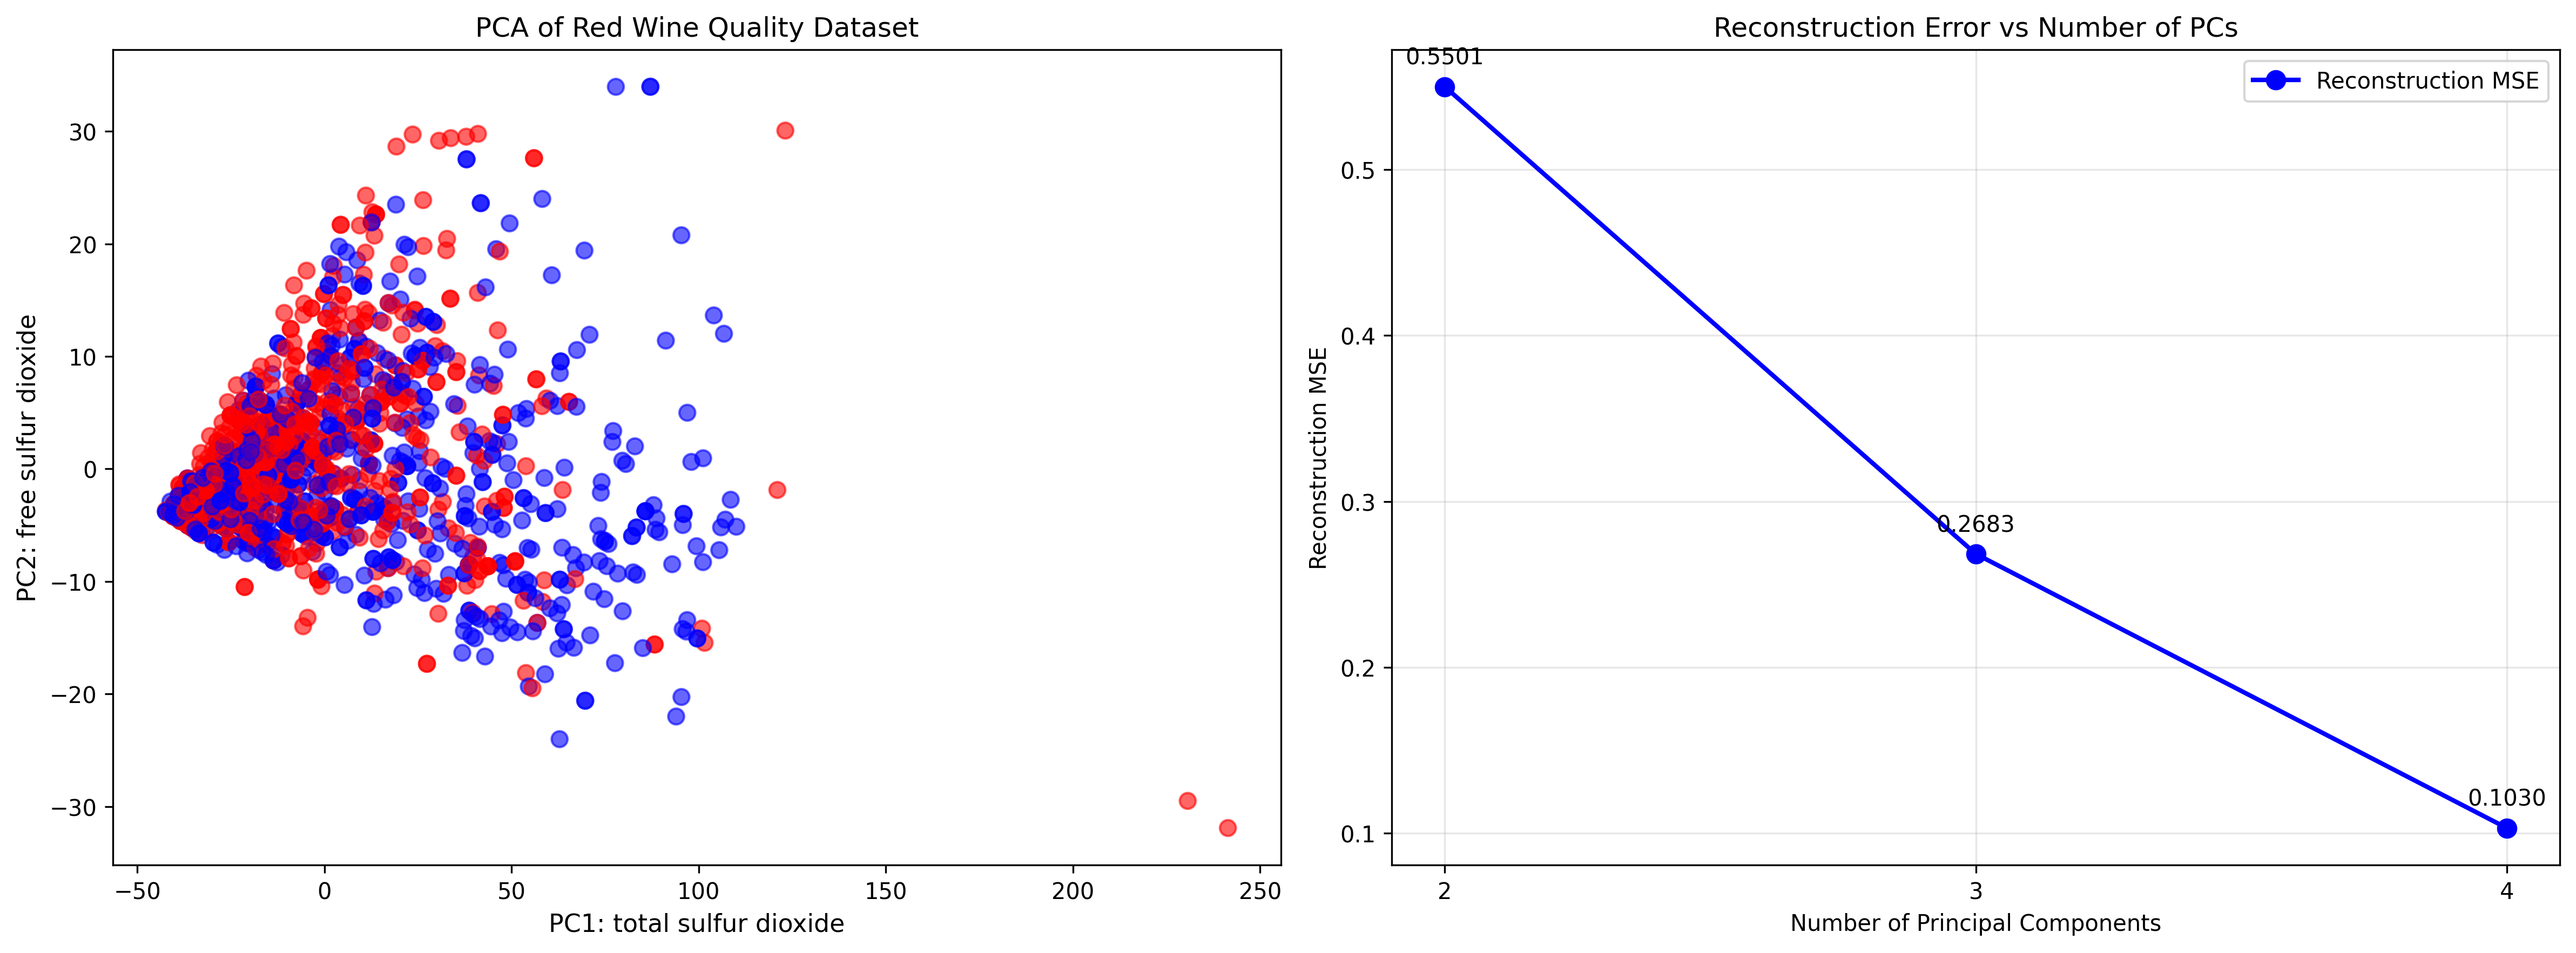
\includegraphics[width=\textwidth]{images/wine_quality_combined_analysis.png}
    \caption{Red Wine Quality Linear Regression Model Plot}\label{fig:red_wine_quality}
\end{figure}

\newpage
\subsubsection{Tabular Outputs}
The results of the \textbf{Linear} Regression model are summarized in Table~\ref{tab:red_wine_quality_results}.

\begin{table}[htbp]
    \centering
    \begin{tabular}{ || l || c || l || }
        \hline
        \textbf{Metric} & \textbf{Value} & \textbf{Interpretation} \\
        \hline\hline
        Cross Validation Scores & [0.270419 0.354977 0.309328] & R² scores for each fold \\
        \hline
        Mean Cross Validation Score & 0.311 & Average R² score \\
        \hline
    \end{tabular}
    \caption{Red Wine Quality Linear Regression Model Results}\label{tab:red_wine_quality_results}
\end{table}

\noindent The results of the \textbf{Logistic} Regression model are summarized in Table~\ref{tab:red_wine_quality_classification}.
\begin{table}[htbp]
    \centering
    \begin{tabular}{ || l || c || l || }
        \hline
        \textbf{Class} & \textbf{Count} & \textbf{Interpretation} \\
        \hline\hline
        Cross Validation Scores & [0.705441 0.733583 0.748593] & R² scores for each fold \\
        \hline
        Mean Cross Validation Score & 0.729 & Average R² score \\
        \hline
    \end{tabular}
    \caption{Red Wine Quality Logistic Regression Model Results}\label{tab:red_wine_quality_classification}
\end{table}

\noindent The PCA results are summarized in Table~\ref{tab:pca_analysis}.
\begin{table}[htbp]
    \centering
    \begin{tabular}{ || l || c || l || }
        \hline
        \textbf{Component} & \textbf{Variance Explained} & \textbf{Top Contributing Features} \\
        \hline\hline
        PC1 & 94.66\% & \begin{tabular}[t]{@{}l@{}}Total sulfur dioxide (0.976) \\ Free sulfur dioxide (0.219)\end{tabular} \\
        \hline
        PC2 & 4.84\% & \begin{tabular}[t]{@{}l@{}}Free sulfur dioxide (0.975) \\ Total sulfur dioxide (-0.219)\end{tabular} \\
        \hline
        Combined PC1+PC2 & 99.49\% & Sulfur dioxide compounds dominate variance \\
        \hline
    \end{tabular}
    \caption{PCA Results for Wine Quality Dataset}\label{tab:pca_analysis}
\end{table}

\noindent The results of using different numbers of principal components is shown in Table~\ref{tab:reconstruction_analysis}.
\begin{table}[h!]
    \centering
    \begin{tabular}{ || l || c || c || c || }
        \hline
        \textbf{Components} & \textbf{MSE} & \textbf{Explained Variance} & \textbf{Reconstruction Error} \\
        \hline\hline
        2 PCs & 0.550 & 99.49\% & 0.51\% \\
        \hline
        3 PCs & 0.268 & 99.75\% & 0.25\% \\
        \hline
        4 PCs & 0.103 & 99.91\% & 0.09\% \\
        \hline
    \end{tabular}
    \caption{PCA Results Using Different Numbers of Principal Components}\label{tab:reconstruction_analysis}
\end{table}

\newpage
\subsubsection{Analysis}
The Red Wine Quality dataset was analyzed using Linear Regression, Logistic Regression, and Principal Component Analysis (PCA).
Both the Linear and Logistic Regression models were evaluated using a three-fold cross-validation approach to determine the model's performance.
The mean R² score across the three folds of the linear model was approximately 0.311, indicating a moderate fit of this model to the data. 
This explains that the linear model is only able to account for \textasciitilde{31.1}\% of the variance in wine quality based on the provided dataset.

The Logistic Regression model, which utilized binary classification of wine quality into ``High'' and ``Low'' categories, resulted in a mean R² score of approximately 0.729 across the three folds.
This indicates that, for this dataset, the logistic model is a better fit than the linear model, explaining \textasciitilde{72.9}\% of the variance in wine quality.
This suggests that the relationship between the features and wine quality is better captured by a classification approach rather than a regression approach.

PCA was performed to determine which features contributed most to the variance in the dataset.
The first two principal components (PC1 and PC2) explained a combined 99.49\% of the variance, with PC1 alone accounting for 94.66\%.
The top contributing features to PC1 were total sulfur dioxide and free sulfur dioxide, indicating that these chemicals are significant factors in determining wine quality.
Using increasing numbers of principal components showed that even with just 2 PCs, the reconstruction error was only 0.51\%, 
indicating that the majority of the information in the dataset can be captured with a very low-dimensional representation (Total Sulfur Dioxide, Free Sulfur Dioxide, Resultant Wine Quality).
Intuition would tell that wine quality is influenced by a combination of factors, not just these two features alone. 
However, PCA identifies the directions of maximum variance in the data, which may not directly correspond to the most intuitive or expected features.